\documentclass{beamer}

\mode<presentation> {
	\usetheme{Madrid}
	\usepackage{graphicx}
	\usepackage{booktabs}
}

%----------------------------------------------------------------------------------------
%	TITLE PAGE
%----------------------------------------------------------------------------------------
\title[Take a Look!]{Take a Look!: Investigating the Relative Contributions of Children's Books and Child-Directed Speech} % The short title appears at the bottom of every slide, the full title is only on the title page

\author{Joseph Denby} % Your name
\institute[] % Your institution as it will appear on the bottom of every slide, may be shorthand to save space
{
	Perspectives on Computational Research \\ % Your institution for the title page
	\medskip
	%\textit{john@smith.com} % Your email address
}
\date{\today} % Date, can be changed to a custom date

\begin{document}
	
	\begin{frame}
		\titlepage % Print the title page as the first slide
		\begin{figure}
			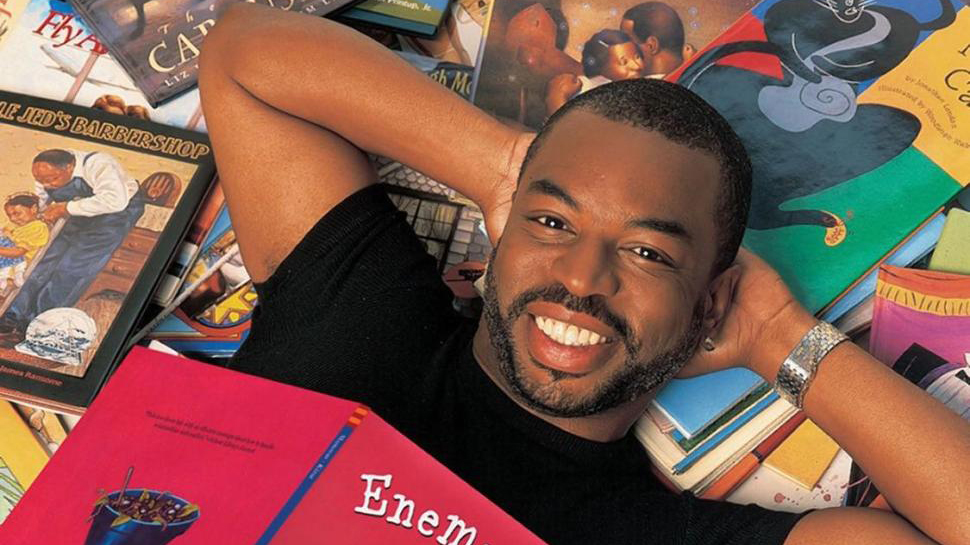
\includegraphics[width=.4\linewidth]{readrainbow.jpg}
		\end{figure}
	\end{frame}
	

%----------------------------------------------------------------------------------------
%	PRESENTATION SLIDES
%----------------------------------------------------------------------------------------
\begin{frame}{Introduction}
	\begin{center}
		\Huge How do we learn language? \\
		\vspace{3mm}
		\small or, more specifically, \\
		\vspace{3mm}
		\Large From what sources do children glean language rules/use and what do they contribute respectively?
	\end{center}
\end{frame}


\begin{frame}{Background}
	\begin{itemize}
		\item Extensive work on child-directed speech (CDS)
		\begin{itemize}
			\item Aspects of CDS predict vocabulary skill (Rowe 2008; Rowe 2012)
			\item CDS linguistic construction differs markedly from standard speech (Cameron-Faulkner et al., 2001)
		\end{itemize}
		\item Recent work investigates children's books as important source
		\begin{itemize}
			\item e.g., Whitehurst et al., 1988; Montag et al., 2015; Montag et al., 2017
		\end{itemize}

	\end{itemize}
\end{frame}

\begin{frame}
	\frametitle{Setup / Objective}
	\begin{itemize}
		
		\item Caregiver speech and picture books are two prominent sources of linguistic input for children
		\item Research has historically neglected the latter
		\item Important to assess their relative (unique?) contributions
		
	\end{itemize}
	\begin{block}{Montag et al.(2015), 2}
		What language-learning data might early picture books provide that everyday conversations do not?
	\end{block}
\end{frame}


\begin{frame}{Objective}
	\small Question for this project: \\
	\begin{center}
		\Large What are substantive differences in the content of child-directed speech and age-appropriate children's books?
	\end{center}
\end{frame}

\begin{frame}
	\frametitle{Procedure}
	\begin{itemize}
		\item Content Analysis on Speech and Text Corpora
		\begin{enumerate}
			\item Relative POS usage across time
			\item Average sentence complexity (using tree parsing)
			\item Lexical diversity through type-token ratio (TTR)
			\item ...etc.
			
		\end{enumerate}
	\end{itemize}
\end{frame}

\begin{frame}
	\frametitle{Corpora --  Language Development Project (LDP)}
	\begin{itemize}
		\item UChicago-based initiative to document parent-child interactions with a socioeconomically-diverse sample ($n=102$)
		\item Ecological check-ins between ages 14 - 58 months at four month intervals
		\item Analysis draws from transcripts of caregiver speech
	\end{itemize}
	\begin{center}
		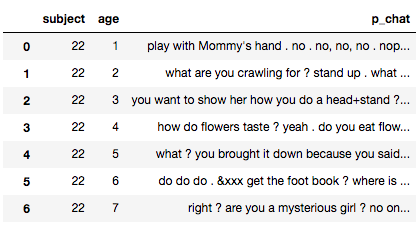
\includegraphics[width=.6\linewidth]{ldp_excerpt.png}
	\end{center}

\end{frame}



\begin{frame}
	\frametitle{Corpora  -- Books}
	\footnotesize{Montag, J. L., Jones, M. N., \& Smith, L. B. (2015). The words children hear: Picture books and the statistics for language learning. Psychological Science, 26, 1489-1496.} 
	\vspace{5mm}
	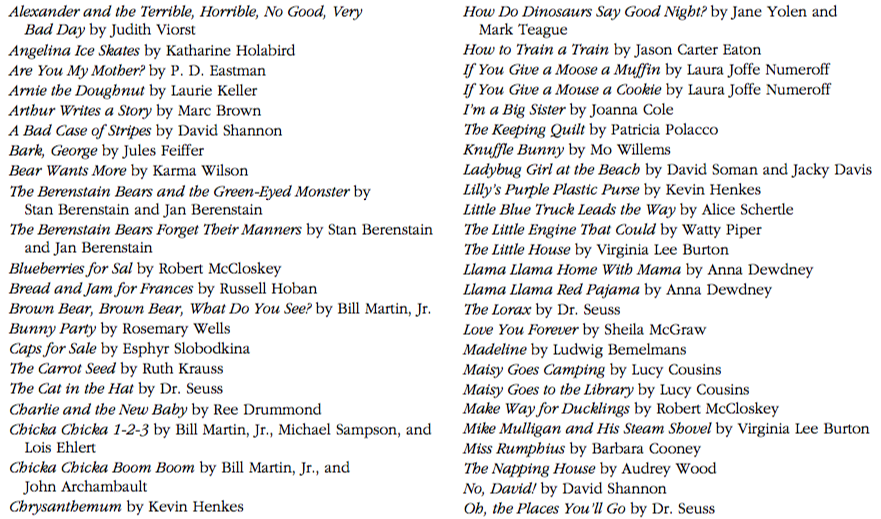
\includegraphics[width=.9\linewidth]{kidbooks.png}
\end{frame}

\begin{frame}{Projections}
	\begin{itemize}
		\item Repicate previous work showing that books exhibit higher TTR (with different speech corpus)
		\item Uncover meaningful distinctions between syntactic make-up of books vs. speech
		\begin{itemize}
			\item Hopefully uncover specific benefits of children's books (and speech)
		\end{itemize}
	\end{itemize}

	
\end{frame}

\begin{frame}{Thank you!}
	\begin{center}
		\Huge Questions?
	\end{center}
\end{frame}
	
	
\end{document}
